% ============================================================
%  Theory and Methodology Report — Photon Shower Shape
%  Cell-Level Reweighting in the ATLAS LAr EM Calorimeter
% ============================================================
\documentclass[11pt,a4paper]{article}

% --- Encoding & fonts ---
\usepackage[utf8]{inputenc}
\usepackage[T1]{fontenc}
\usepackage{lmodern}

% --- Page layout ---
\usepackage[margin=2.5cm]{geometry}

% --- Math ---
\usepackage{amsmath,amssymb,mathtools}

% --- Graphics ---
\usepackage{graphicx}
\usepackage{xcolor}
\graphicspath{%
  {../output/Layer_1/eta_loose/llgamma/unconverted/plots/}%
  {../output/Layer_2/eta_loose/llgamma/unconverted/plots/}%
}

% --- Tables ---
\usepackage{booktabs}
\usepackage{longtable}
\usepackage{array}
\usepackage{multirow}

% --- Captions & floats ---
\usepackage{caption}
\usepackage{subcaption}
\usepackage{float}

% --- TikZ & PGF ---
\usepackage{tikz}
\usetikzlibrary{calc,decorations.pathreplacing,arrows.meta,patterns,
                shapes.geometric,positioning,fit,backgrounds}
\usepackage{pgfplots}
\pgfplotsset{compat=1.18}

% --- Units ---
\usepackage{siunitx}
\sisetup{separate-uncertainty=true,range-phrase=\,--\,}

% --- Hyperlinks ---
\usepackage[colorlinks=true,linkcolor=blue!60!black,
            citecolor=green!50!black,urlcolor=blue!70!black]{hyperref}
\usepackage{cleveref}

% --- Bibliography ---
\usepackage[backend=biber,style=numeric-comp,sorting=none,
            maxnames=6,giveninits=true]{biblatex}
\addbibresource{refs_theory.bib}

% --- Misc ---
\usepackage{microtype}
\usepackage{parskip}
\usepackage{enumitem}

% ============================================================
%  Custom commands
% ============================================================
\newcommand{\Reta}{R_{\eta}}
\newcommand{\Rphi}{R_{\phi}}
\newcommand{\weta}{w_{\eta 2}}
\newcommand{\wetaone}{w_{\eta 1}}
\newcommand{\wstot}{w_{s,\mathrm{tot}}}
\newcommand{\fside}{f_{\mathrm{side}}}
\newcommand{\dE}{\Delta E}
\newcommand{\Eratio}{E_{\mathrm{ratio}}}
\newcommand{\abseta}{|\eta|}
\newcommand{\chisq}{\chi^2/N_\mathrm{bins}}
\newcommand{\pt}{p_{\mathrm{T}}}
\newcommand{\Xnaught}{X_0}
\newcommand{\RM}{R_\mathrm{M}^{\phantom{0}}}
\newcommand{\avgmu}{\langle\mu\rangle}
\newcommand{\Elr}[1]{E_{\mathrm{Lr#1}}}

% ============================================================
\begin{document}

\begin{titlepage}
  \centering
  \vspace*{2cm}
  {\LARGE\bfseries Cell-Level Shower Shape Reweighting\\[0.4em]
   in the ATLAS LAr EM Calorimeter:\\[0.4em]
   Theory, Methodology, and Outlook\par}
  \vspace{1.5cm}
  {\large Marta Fernandez Silva\\[0.3em]
   ATLAS QT Working Group\\[0.3em]
   April 2026\par}
  \vspace{2cm}
  \begin{abstract}
    \noindent
    Shower-shape variables computed from electromagnetic (EM) calorimeter cells
    are central to photon identification in the ATLAS experiment and to precision
    measurements such as the Higgs CP-structure combination.  Systematic
    discrepancies between data and Monte Carlo (MC) simulation in these variables
    propagate directly into photon-identification efficiencies and into the
    modelling of inputs to machine-learning classifiers that operate at the
    cell level.  This report provides a self-contained, pedagogical treatment
    of the origin of these discrepancies, the cell-level reweighting methodology
    developed to correct them, and a detailed analysis of why Layer~1 of the
    LAr accordion calorimeter presents substantially greater challenges than
    Layer~2.  Concrete proposals for binning optimisation, alternative
    correction strategies (normalising flows, classifier-based reweighting,
    optimal transport, and diffusion models), and actionable next steps are
    presented.
  \end{abstract}
  \vfill
  {\small\textit{Internal note — not for public distribution.}}
\end{titlepage}

\tableofcontents
\newpage

% ============================================================
\section{Introduction}
\label{sec:intro}
% ============================================================

The ATLAS detector~\cite{ATLAS:2008} at the Large Hadron Collider (LHC)
reconstructs photons primarily through their energy deposits in the
liquid-argon (LAr) electromagnetic (EM) calorimeter.  The
characteristic lateral and longitudinal profile of an electromagnetic
shower encodes the identity of the initiating particle and, at
sufficient resolution, carries information about its production
mechanism.  A set of \emph{shower shape variables} — scalar summaries
of the cell-energy distribution within a fixed calorimeter window — is
the traditional foundation of photon identification in
ATLAS~\cite{ATLAS:photonID2019,ATLAS:photonID2022}.

Recent analyses push beyond scalar summaries: deep convolutional
networks~\cite{ATLAS:CaloCellML} and graph neural networks now
consume raw cell energies, making the accurate simulation of
\emph{individual cell responses} a prerequisite rather than a
convenience.  The Higgs boson CP-structure combination that motivates
the present work involves several Higgs decay channels, each relying
on tight photon identification whose efficiency uncertainty feeds
directly into the measurement's systematic budget.

Simulated events in ATLAS are produced with \textsc{Geant4}~\cite{Geant4:2003}
interfaced to the ATLAS detector model.  Despite the sophistication of
this simulation, residual discrepancies between data and MC
distributions in shower-shape variables are well established and are
corrected empirically via \emph{fudge factors}~\cite{ATLAS:fudgePub}:
additive offsets applied to each variable after reconstruction.  Fudge
factors are a successful but coarse instrument.  They
\begin{enumerate}[label=(\roman*)]
  \item perturb the variable value without correcting the underlying
        cell-energy distribution,
  \item cannot simultaneously correct correlated pairs of variables
        (e.g.\ $\Reta$ and $\weta$),
  \item cannot improve the modelling of ML classifiers that bypass
        high-level variables altogether.
\end{enumerate}
A cell-level reweighting approach directly modifies the per-cell
energy fractions of simulated photon clusters before any high-level
variable is computed, addressing all three limitations.

This report is organised as follows.
\Cref{sec:atlas} describes the ATLAS detector and the LAr EM
calorimeter in the detail required for the methodology.
\Cref{sec:variables} defines all shower-shape variables studied.
\Cref{sec:discrepancy} discusses the physical origin of data/MC
discrepancies.
\Cref{sec:method} presents the cell-level reweighting methodology in
full technical detail, including the two-pass pipeline, the
hot-cell recentering algorithm, and the padding treatment.
\Cref{sec:layer1} analyses why Layer~1 corrections are substantially
harder to derive than Layer~2 corrections, supported by quantitative
$\chisq$ comparisons.
\Cref{sec:binning} proposes binning optimisations to improve the
current correction scheme.
\Cref{sec:alternatives} surveys alternative methodologies from the
machine-learning literature.
\Cref{sec:conclusions} collects conclusions and concrete action items.
Appendices provide reference tables, formula compendiums, and
code pointers.

% ============================================================
\section{The ATLAS Detector and the LAr EM Calorimeter}
\label{sec:atlas}
% ============================================================

\subsection{Detector Overview}
\label{sec:atlas:overview}

The ATLAS detector~\cite{ATLAS:2008} is a multipurpose particle
detector with a forward-backward symmetric cylindrical geometry
covering nearly the full $4\pi$ solid angle around the interaction
point.  It consists, from inside out, of an inner tracking detector
(ID), electromagnetic and hadronic calorimeters, and a muon
spectrometer, all embedded in toroidal and solenoid magnetic fields.
The coordinate system uses a right-handed frame with the $z$-axis
along the beam pipe; the azimuthal angle $\phi$ is measured around
the beam axis and the pseudorapidity $\eta = -\ln[\tan(\theta/2)]$
replaces the polar angle $\theta$.  Transverse momentum
$\pt = p\sin\theta$ and transverse energy $E_\mathrm{T} = E\sin\theta$
are defined in the transverse plane.

\subsection{Liquid-Argon EM Calorimeter Geometry}
\label{sec:atlas:lar}

The LAr EM calorimeter~\cite{LArTDR:1996,ATLAS:LAr_Run3} is a
lead/liquid-argon sampling calorimeter with an accordion-shaped
absorber structure (\cref{fig:accordion}).  It is divided into a
barrel section ($\abseta < 1.475$) and two end-cap sections
($1.375 < \abseta < 3.2$).  The accordion geometry provides
complete and uniform $\phi$ coverage without azimuthal cracks.

\begin{figure}[htbp]
  \centering
  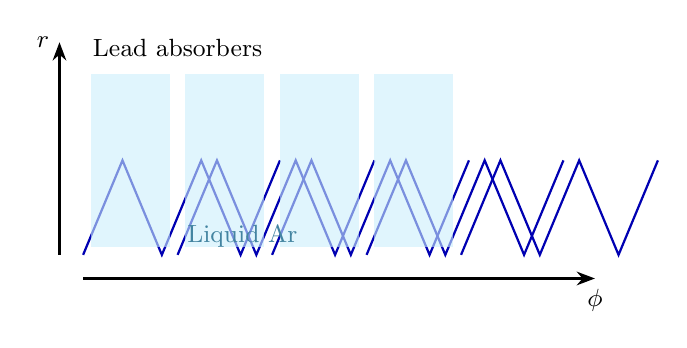
\begin{tikzpicture}[scale=1.0]
    % Draw an accordion-style zig-zag representing the LAr absorber structure
    \def\amp{0.5}   % amplitude
    \def\freq{1.2}  % spatial frequency scale
    \def\depth{5.0} % radial depth
    \def\nlayers{4} % number of absorber layers shown
    \foreach \k in {0,1,2,3,4} {
      \draw[thick,blue!70!black] (\k*1.2, 0)
        -- ++(\amp,  \freq) -- ++(\amp, -\freq)
        -- ++(\amp,  \freq) -- ++(\amp, -\freq)
        -- ++(\amp,  \freq);
    }
    % LAr gaps (blue fill between absorbers)
    \foreach \k in {0,1,2,3} {
      \fill[cyan!20,opacity=0.6]
        (\k*1.2+0.1, 0.1) rectangle (\k*1.2+1.1, \freq*2-0.1);
    }
    % Labels
    \node[above right, font=\small] at (0, \freq*2) {Lead absorbers};
    \node[below right, font=\small, cyan!60!black] at (1.2, 0.5)
      {Liquid Ar};
    % Arrow indicating radial direction
    \draw[-{Stealth},thick] (-0.3, 0) -- (-0.3, \freq*2+0.3)
      node[left,font=\small] {$r$};
    \draw[-{Stealth},thick] (0, -0.3) -- (6.5, -0.3)
      node[below,font=\small] {$\phi$};
  \end{tikzpicture}
  \caption{Schematic cross-section of the accordion structure of the
           ATLAS LAr EM calorimeter (not to scale).  Lead absorber
           plates (blue) are interleaved with liquid-argon gaps
           (cyan).  The accordion fold geometry provides uniform
           $\phi$ coverage without azimuthal cracks.}
  \label{fig:accordion}
\end{figure}

The EM calorimeter is longitudinally segmented into four layers for
$\abseta < 2.5$ (the precision measurement region):
a thin \emph{presampler} (PS, also called Layer~0) that corrects
for upstream energy loss, a finely segmented \emph{first sampling
layer} (Layer~1 or ``strip layer''), a thick \emph{second sampling
layer} (Layer~2) containing most of the shower energy, and a
coarser \emph{third sampling layer} (Layer~3 or L3).
\Cref{tab:granularity} summarises the cell granularity in each
layer for the barrel and end-cap regions.

\begin{table}[htbp]
  \centering
  \caption{LAr EM calorimeter cell granularity
           $\Delta\eta \times \Delta\phi$ in each sampling layer
           for selected pseudorapidity ranges~\cite{ATLAS:2008}.
           Values are given as $\Delta\eta \times \Delta\phi$.}
  \label{tab:granularity}
  \begin{tabular}{llcc}
    \toprule
    Layer & Region & $\Delta\eta \times \Delta\phi$ & Depth [$X_0$] \\
    \midrule
    Presampler (PS) & $\abseta < 1.52$ & $0.025 \times 0.1$ & $\sim 1.5$ \\
    Presampler (PS) & $1.5 < \abseta < 1.8$ & $0.025 \times 0.1$ & $\sim 1.5$ \\
    \midrule
    Layer~1 (strips) & $\abseta < 1.40$ & $0.003125 \times 0.1$ & $4.3$ \\
    Layer~1 (strips) & $1.40 < \abseta < 1.475$ & $0.025 \times 0.025$ & $4.3$ \\
    Layer~1 (strips) & $1.5 < \abseta < 1.8$ & $0.025 \times 0.1$ & $4.3$ \\
    Layer~1 (strips) & $1.8 < \abseta < 2.0$ & $0.0125 \times 0.1$ & $4.3$ \\
    Layer~1 (strips) & $2.0 < \abseta < 2.4$ & $0.00625 \times 0.1$ & $4.3$ \\
    Layer~1 (strips) & $2.4 < \abseta < 2.5$ & $0.025 \times 0.1$ & $4.3$ \\
    \midrule
    Layer~2 & $\abseta < 1.40$ & $0.025 \times 0.025$ & $16$ \\
    Layer~2 & $1.40 < \abseta < 1.475$ & $0.075 \times 0.025$ & $16$ \\
    Layer~2 & $1.5 < \abseta < 2.5$ & $0.025 \times 0.025$ & $16$ \\
    \midrule
    Layer~3 & $\abseta < 1.35$ & $0.050 \times 0.025$ & $2$ \\
    Layer~3 & $1.5 < \abseta < 2.5$ & $0.050 \times 0.025$ & $2$ \\
    \bottomrule
  \end{tabular}
\end{table}

\subsubsection{Layer~1 (Strip Layer)}
\label{sec:atlas:layer1}

Layer~1 is the most finely segmented layer in the $\eta$ direction:
in the barrel region ($\abseta < 1.4$) each cell spans only
$\Delta\eta \approx 0.003125$ compared with $\Delta\phi = 0.1$,
yielding an aspect ratio of $\approx 32{:}1$.  This extreme
segmentation is designed to resolve the two-photon decay of
$\pi^0 \to \gamma\gamma$ — the dominant source of fake photons — from
genuine prompt photons: a $\pi^0$ produces two nearby showers
separated in $\eta$ by $\sim$$\Delta\eta_{\pi^0} \propto
m_{\pi^0}/(2p_\mathrm{T})$, whereas a genuine photon produces a
single narrow shower.  The strip layer thus provides
\emph{fine-grained longitudinal shower profile information} in the
earliest part of the electromagnetic shower where pair-production
dominates.

The trade-off for this fine segmentation is a very small
signal-to-noise ratio per cell: for a typical photon with
$\pt \sim 40$~GeV, the energy deposited in an individual strip cell
is $\mathcal{O}(100\,\mathrm{MeV})$ compared with an electronic noise
of $\mathcal{O}(50\text{--}100\,\mathrm{MeV})$~\cite{LArTDR:1996}.

\subsubsection{Layer~2 (Main Sampling Layer)}
\label{sec:atlas:layer2}

Layer~2 contains approximately $16\,X_0$ of material and captures
$\sim$80\% of the total shower energy.  Each cell spans
$\Delta\eta \times \Delta\phi = 0.025 \times 0.025$ — a nearly
square geometry.  The signal-to-noise ratio per cell is
significantly more favourable than in Layer~1 because the cells are
larger and collect more energy.

\subsubsection{Shower Cluster Reconstruction}
\label{sec:atlas:cluster}

Photon energy is measured from a fixed-size \emph{sliding-window
supercluster} of $N_\eta \times N_\phi = 3 \times 5$~Layer-2 cells
in the barrel (energy seed) and a larger $5 \times 5$ window in the
end-cap~\cite{ATLAS:egammaReco2019,ATLAS:egammaRun3}.  The
longitudinal cluster used in shower-shape computation spans
$7 \times 11$ Layer-2 cell units across all layers; this defines
the reweighting window used in the present work.  In Layer~2, this
corresponds to a window of $7 \times 11 = 77$ cells
($0.175 \times 0.275$ in $\eta \times \phi$), while in Layer~1 the
same angular window maps to $56 \times 2 = 112$ strip cells
(the Layer-1 $\phi$ segmentation is 5$\times$ coarser than Layer~2).

\subsection{Electromagnetic Shower Physics}
\label{sec:atlas:shower}

An electromagnetic shower is initiated when a high-energy photon or
electron enters the calorimeter absorber material.  Above the
critical energy $E_c$ (approximately $7.3$~MeV in lead~\cite{PDG:2024}),
the dominant processes are pair production
($\gamma \to e^+e^-$) and bremsstrahlung ($e^\pm \to e^\pm\gamma$).
These processes cascade into a multiplication of secondary particles,
each with half the energy of its parent, until the individual particle
energies fall below $E_c$, after which ionisation dominates and the
shower terminates.

The longitudinal shower profile is well described by a gamma distribution
in units of radiation length $\Xnaught$:
\begin{equation}
  \frac{\mathrm{d}E}{\mathrm{d}t} = E_0\,b\,
    \frac{(bt)^{a-1}\,e^{-bt}}{\Gamma(a)}\,,
  \label{eq:shower:long}
\end{equation}
where $t = x/\Xnaught$ is the shower depth in units of $\Xnaught$,
$a$ and $b$ are shape parameters that depend on the particle energy
and the absorber material, and the shower maximum occurs at
$t_\mathrm{max} = (a-1)/b \approx \ln(E_0/E_c) - 0.5$ for photons.
For a typical 40~GeV photon in lead, $t_\mathrm{max} \approx 8\,\Xnaught$,
placing the shower maximum well inside Layer~2
($\approx 16\,\Xnaught$ thick) after traversing the presampler
($\approx 1.5\,\Xnaught$) and Layer~1 ($\approx 4\,\Xnaught$).

The transverse shower profile at depth $t$ is approximately a sum of
two Gaussian components~\cite{PDG:2024}:
\begin{equation}
  \frac{1}{E}\frac{\mathrm{d}E}{\mathrm{d}r} =
    \frac{(1-f_\mathrm{core})}{2\pi\sigma_c^2}
    e^{-r^2/(2\sigma_c^2)} +
    \frac{f_\mathrm{core}}{2\pi\sigma_t^2}
    e^{-r^2/(2\sigma_t^2)}\,,
  \label{eq:shower:trans}
\end{equation}
where $r$ is the transverse distance from the shower axis,
$\sigma_c \sim 0.5\,\RM$ is the narrow core width,
$\sigma_t \sim 2\,\RM$ is the wider tail width, and
$f_\mathrm{core}$ is the fractional amplitude of the tail component.
The Moli\`ere radius $\RM$ (approximately $1.6$~cm in lead) sets
the transverse scale of 90\% containment.
In the barrel calorimeter, $\RM$ corresponds to approximately 3 Layer-2
cells in $\eta$.

The fine $\eta$ granularity of Layer~1 resolves the \emph{longitudinal
shower profile before the shower maximum} — the region most
sensitive to the two-subjet topology of $\pi^0$ decays
(\cref{fig:shower_profile}).

\begin{figure}[htbp]
  \centering
  \begin{tikzpicture}[scale=0.9]
    % Draw a simplified longitudinal shower profile
    % X-axis = depth in X0, Y-axis = dE/dt
    \begin{axis}[
      width=9cm, height=5.5cm,
      xlabel={Shower depth $t = x/X_0$},
      ylabel={$\mathrm{d}E/\mathrm{d}t$ [a.u.]},
      xmin=0, xmax=30,
      ymin=0, ymax=1.2,
      xtick={0,5,10,15,20,25,30},
      every axis plot/.append style={line width=1.2pt},
      legend style={at={(0.95,0.95)},anchor=north east,font=\small},
    ]
    % Gamma distribution profile: a=7.5, b=0.9 (typical photon)
    \addplot[domain=0.1:30, samples=200, blue!70!black] {
      ( (0.9*x)^(7.5-1) * exp(-0.9*x) ) /
      exp(ln(6.5)+6.5*ln(0.9)-0.9*0+0) * 2.5
    };
    % Shaded layer regions
    \addplot[fill=gray!20,draw=none,forget plot] coordinates
      {(0,0)(1.5,0)(1.5,1.2)(0,1.2)} \closedcycle;
    \addplot[fill=blue!10,draw=none,forget plot] coordinates
      {(1.5,0)(5.8,0)(5.8,1.2)(1.5,1.2)} \closedcycle;
    \addplot[fill=green!10,draw=none,forget plot] coordinates
      {(5.8,0)(21.8,0)(21.8,1.2)(5.8,1.2)} \closedcycle;
    \addplot[fill=orange!10,draw=none,forget plot] coordinates
      {(21.8,0)(23.8,0)(23.8,1.2)(21.8,1.2)} \closedcycle;
    % Labels
    \node[font=\tiny] at (axis cs: 0.75, 1.1) {PS};
    \node[font=\tiny] at (axis cs: 3.65, 1.1) {L1};
    \node[font=\tiny] at (axis cs: 13.8, 1.1) {L2};
    \node[font=\tiny] at (axis cs: 22.8, 1.1) {L3};
    % Redraw profile on top
    \addplot[domain=0.1:30, samples=200, blue!70!black, thick] {
      0.95 * ( (0.9*x)^6.5 * exp(-0.9*x) ) /
      ((0.9*16.4)^6.5 * exp(-0.9*16.4)) * 1.15
    };
    \legend{$\mathrm{d}E/\mathrm{d}t$ (EM shower)}
    \end{axis}
  \end{tikzpicture}
  \caption{Schematic longitudinal shower energy profile
           (gamma-distribution model, \cref{eq:shower:long})
           overlaid with the approximate LAr calorimeter layer
           boundaries (PS, L1, L2, L3) in units of radiation
           length $X_0$ for a 40~GeV photon in the barrel.
           Layer~1 samples the rising edge of the shower, before
           the maximum, where the profile is most sensitive to
           two-photon substructure from $\pi^0 \to \gamma\gamma$.}
  \label{fig:shower_profile}
\end{figure}


% ============================================================
\section{Shower Shape Variables}
\label{sec:variables}
% ============================================================

Shower-shape variables are scalar quantities computed from the energy
deposits in one or more calorimeter layers within a fixed rectangular
window centred on the photon cluster.  They encode the lateral and
longitudinal spread of the shower and are the primary discriminants
used in the ATLAS photon identification working
points~\cite{ATLAS:photonID2019,ATLAS:photonID2022}.  The variables
most relevant to this study are defined below.

\subsection{Layer~2 Variables}
\label{sec:variables:layer2}

Let $E_{i,j}$ denote the energy deposited in the cell at position
$(i, j)$ in a $\eta \times \phi$ grid centred on the shower
barycentre, where $i$ runs over $\eta$ and $j$ over $\phi$.

\subsubsection{Lateral containment ratio \texorpdfstring{$\Reta$}{Reta}}

\begin{equation}
  \Reta = \frac{\sum_{|i|\le 3, |j|\le 2} E_{i,j}}
               {\sum_{|i|\le 7, |j|\le 2} E_{i,j}}
  \label{eq:reta}
\end{equation}
$\Reta$ is the fraction of the cluster energy in a $3\times 7$
window relative to a $7\times 7$ window in Layer~2
(in $\eta \times \phi$ cells of size $0.025 \times 0.025$).
A genuine photon shower is narrow in $\eta$ ($\Reta \to 1$), while
a hadronic fake or a $\pi^0 \to \gamma\gamma$ is broader ($\Reta <
0.92$ for typical rejection working points).

\subsubsection{Azimuthal containment ratio \texorpdfstring{$\Rphi$}{Rphi}}

\begin{equation}
  \Rphi = \frac{\sum_{|i|\le 3, |j|\le 2} E_{i,j}}
               {\sum_{|i|\le 3, |j|\le 3} E_{i,j}}
  \label{eq:rphi}
\end{equation}
$\Rphi$ measures the lateral containment in the $\phi$ direction.
Because the shower shape is nearly symmetric in $\phi$, $\Rphi$
is less discriminating than $\Reta$ but provides complementary
information about the $\phi$ spread.

\subsubsection{Second moment of lateral shower width \texorpdfstring{$\weta$}{weta2}}

\begin{equation}
  \weta = \sqrt{\frac{\sum_i E_i \eta_i^2}{\sum_i E_i}
               - \left(\frac{\sum_i E_i \eta_i}{\sum_i E_i}\right)^2}
  \label{eq:weta2}
\end{equation}
The sum runs over cells in a $3\times 5$ window.  $\weta$ is the
energy-weighted second moment (standard deviation) of the cell $\eta$
positions.  It is sensitive to the overall width of the shower and
directly related to the core component width $\sigma_c$ in
\cref{eq:shower:trans}.

\subsection{Layer~1 Variables}
\label{sec:variables:layer1}

Layer~1 variables exploit the fine $\eta$ segmentation (strip cells)
to probe the two-subjet topology of $\pi^0$ decays.  The window used
in the barrel is $\Delta\eta_\mathrm{window} = 0.0625$,
corresponding to $20$ strips.  Variables are computed relative to
the strip barycentre.

\subsubsection{Shower width in strips \texorpdfstring{$\wetaone$}{weta1}}

\begin{equation}
  \wetaone = \sqrt{
    \frac{\sum_i E_i \eta_i^2}{\sum_i E_i}
    - \left(\frac{\sum_i E_i \eta_i}{\sum_i E_i}\right)^2}
  \label{eq:wetaone}
\end{equation}
The sum runs over all strip cells in the $\pm 10$-strip window
centred on the barycentre.  $\wetaone$ is the Layer-1 analogue of
$\weta$: it measures the overall $\eta$ width of the energy deposit
in the strip layer.

\subsubsection{Total transverse width \texorpdfstring{$\wstot$}{wstot}}

\begin{equation}
  \wstot = \sqrt{
    \frac{\sum_i E_i (i - \bar{i})^2}{\sum_i E_i}}
  \label{eq:wstot}
\end{equation}
The sum now runs over a wider window of $\pm 20$ strips around the
cluster centre.  $\wstot$ is more sensitive to wide secondary
deposits far from the shower core, characteristic of hadronic
contamination or two-photon overlap.

\subsubsection{Side fraction \texorpdfstring{$\fside$}{fside}}

\begin{equation}
  \fside = \frac{
    E(-7, -3) + E(3, 7)}{E(-7, 7)}
  \label{eq:fside}
\end{equation}
where $E(a, b)$ denotes the summed energy over strips $a$ through
$b$ relative to the barycentre strip.  $\fside$ measures the
fraction of the layer-1 energy deposited in the ``side'' strips
outside the central $\pm 2$ strip window.  Genuine photons
concentrate energy in a single narrow peak ($\fside \approx 0$),
while $\pi^0 \to \gamma\gamma$ events produce two separated peaks
resulting in larger $\fside$.

\subsubsection{Energy difference \texorpdfstring{$\dE$}{Delta E}}

\begin{equation}
  \dE = E_\mathrm{2nd\,max} - E_\mathrm{min}
  \label{eq:deltae}
\end{equation}
$\dE$ is the energy difference between the second-largest local
maximum in the strip profile and the energy minimum between the
two maxima.  A non-zero $\dE$ with a local minimum between two
peaks is the smoking-gun signature of a resolved
$\pi^0 \to \gamma\gamma$ decay.  For genuine photons,
$\dE \approx 0$ (single peak).

\subsubsection{Energy ratio \texorpdfstring{$\Eratio$}{Eratio}}

\begin{equation}
  \Eratio = \frac{E_\mathrm{1st\,max} - E_\mathrm{2nd\,max}}
                  {E_\mathrm{1st\,max} + E_\mathrm{2nd\,max}}
  \label{eq:eratio}
\end{equation}
$\Eratio$ is a normalised asymmetry between the two largest
strip-layer energy maxima.  For a genuine photon (single peak),
$\Eratio \to 1$.  For a $\pi^0$ with two resolved sub-showers of
comparable energy, $\Eratio \approx 0$.  $\Eratio$ is dimensionless,
bounded in $[0, 1]$, and arguably the single most powerful
$\pi^0$-rejection variable in Layer~1.

\subsection{Summary and Correlations}
\label{sec:variables:correlations}

\Cref{tab:variables} summarises all variables studied.  The six
Layer-1 variables are strongly correlated among themselves because
they are all derived from the same strip-layer cell-energy
distribution.  A correction of the \emph{cell energies} automatically
corrects all derived variables self-consistently, whereas individual
fudge factors cannot maintain the correct inter-variable covariance.
This motivates the cell-level approach.

\begin{table}[htbp]
  \centering
  \caption{Summary of shower-shape variables studied, their calorimeter
           layer, definition window, and the primary physics they probe.}
  \label{tab:variables}
  \begin{tabular}{lllp{5.5cm}}
    \toprule
    Variable & Layer & Window & Physics probed \\
    \midrule
    $\Reta$    & 2 & $3\times 7$ / $7\times 7$ & Lateral $\eta$ containment\\
    $\Rphi$    & 2 & $3\times 5$ / $3\times 7$ & Lateral $\phi$ containment\\
    $\weta$    & 2 & $3\times 5$               & Shower $\eta$ width (core)\\
    \midrule
    $\wetaone$ & 1 & $\pm 10$ strips           & Overall strip width\\
    $\wstot$   & 1 & $\pm 20$ strips           & Total strip width (tails)\\
    $\fside$   & 1 & $\pm 7$ strips            & Side energy fraction\\
    $\dE$      & 1 & $\pm 10$ strips           & 2nd-max/min energy diff.\\
    $\Eratio$  & 1 & $\pm 2$ strips around max & Asymmetry of two maxima\\
    \bottomrule
  \end{tabular}
\end{table}

% ============================================================
\section{Origin of Data/MC Discrepancies}
\label{sec:discrepancy}
% ============================================================

\subsection{The Simulation Chain}
\label{sec:discrepancy:chain}

ATLAS MC events are produced with a multi-step simulation chain:
\begin{enumerate}[label=\arabic*.]
  \item \textbf{Matrix-element generation}: Hard-scatter processes are
        computed at leading order (LO) or next-to-leading order (NLO)
        using generators such as \textsc{Powheg}~\cite{Powheg:2004},
        \textsc{Sherpa}~\cite{Sherpa:2009}, or
        \textsc{MadGraph}~\cite{PDG:2024}.
  \item \textbf{Parton shower and hadronisation}:
        \textsc{Pythia8}~\cite{Pythia8:2015} or \textsc{Sherpa}
        handle the parton shower, fragmentation, and underlying event.
  \item \textbf{Full detector simulation}: \textsc{Geant4}~\cite{Geant4:2003}
        propagates all stable particles through the ATLAS detector
        geometry, simulating all electromagnetic and hadronic
        interactions.
  \item \textbf{Digitisation}: The simulated ionisation signals are
        converted to ADC counts using a model of the electronics
        response, noise, and pile-up overlaid from minimum-bias
        interactions.
  \item \textbf{Reconstruction}: The same reconstruction algorithms
        used for data are applied to the simulated ADC counts.
\end{enumerate}

Each step introduces potential sources of discrepancy.  Step~3
(\textsc{Geant4}) and Step~4 (digitisation) are the primary sources
of shower-shape mis-modelling.

\subsection{Physical Sources of Mis-modelling}
\label{sec:discrepancy:sources}

\paragraph{Dead material model.}
Passive material upstream of the calorimeter (inner detector,
services, cryostat walls) affects the shower development before the
active volume is reached.  The material budget is measured from
$E/p$ and $Z \to ee$ studies but carries uncertainties of
$\mathcal{O}$(few percent) in radiation lengths.  Upstream showers
initiated in dead material are not perfectly reproduced by the
\textsc{Geant4} geometry model, which leads to a systematic broadening
or narrowing of the shower when it enters the calorimeter active
layers.

\paragraph{Cross-talk between cells.}
Capacitive cross-talk between adjacent strip cells in Layer~1 causes
a fraction of the charge deposited in one cell to appear in its
neighbours.  The cross-talk fraction is measured \emph{in situ} but
is difficult to model accurately at the cell level; it systematically
widens the apparent strip profile.  In MC simulation, the cross-talk
is modelled with a simplified transfer matrix, which may differ from
the true per-channel cross-talk coefficients.

\paragraph{High-voltage (HV) non-uniformities.}
Each LAr cell requires a precisely regulated high voltage to maintain
the correct drift field for the ionisation electrons.  Dead or
degraded HV sectors alter the collected charge and effective cell
gain.  The ATLAS detector database records the HV map per run period,
and corrections are applied in both data and MC, but residual
mis-calibration can contribute to cell-level discrepancies.

\paragraph{Geant4 physics lists.}
The shower development in absorber material depends on the choice
of electromagnetic physics processes in \textsc{Geant4} (energy
thresholds for $\delta$-ray production, Landau fluctuations, Compton
scattering cross-sections).  The ATLAS simulation uses a dedicated
physics list (FTFP\_BERT) tuned to reproduce calorimeter
test-beam data, but residual differences remain, particularly for
the tails of the shower distribution.

\paragraph{Pile-up.}
At high luminosity, many $pp$ interactions occur per bunch crossing
($\avgmu \sim 30$--$60$ in Run~3).  Pile-up deposits energy in
otherwise empty calorimeter cells.  While mean pile-up levels are
reweighted in MC to match data, the local cell-by-cell distribution
of pile-up energy introduces a pedestal that broadens shower-shape
distributions.  This effect is especially significant in
Layer~1 where signal-to-noise is already marginal.

\subsection{The Fudge Factor Approach and Its Limitations}
\label{sec:discrepancy:fudge}

The ATLAS standard correction~\cite{ATLAS:fudgePub} applies
additive offsets (fudge factors) to each shower-shape variable
after reconstruction:
\begin{equation}
  X_\mathrm{corrected} = X_\mathrm{MC} + \Delta X(\eta, E_\mathrm{T})\,,
  \label{eq:fudge}
\end{equation}
where $\Delta X$ is measured from a control sample of photons from
$Z \to \ell\ell\gamma$ or $E/p$-selected electrons, binned in
$\eta$ and $E_\mathrm{T}$.  The fudge factors successfully reduce
the mean residual bias between data and MC but have three structural
limitations:
\begin{enumerate}[label=(\roman*)]
  \item \textbf{Variable-by-variable}: Each variable receives an
        independent offset without constraint from the others.  The
        corrected MC distribution can therefore have the correct
        mean but an inconsistent covariance structure compared with
        data.
  \item \textbf{Distribution shape}: The offset shifts the entire
        distribution rigidly, without adjusting its shape
        (variance, skewness, or higher moments).  The tails of
        distributions — critical for efficiency estimation at tight
        working points — may remain mis-modelled.
  \item \textbf{Cell-level independence}: Fudge factors are applied
        after all cell-energy information has been aggregated into a
        scalar.  They cannot improve the per-cell modelling used by
        ML classifiers or cell-level studies.
\end{enumerate}

The cell-level reweighting method described in \cref{sec:method}
corrects all three limitations by operating directly on the
per-cell energy fractions before any high-level variable is
computed.


% ============================================================
\section{Cell-Level Reweighting Methodology}
\label{sec:method}
% ============================================================

\subsection{Control Sample Selection}
\label{sec:method:selection}

The corrections are derived from a high-purity photon control sample
obtained from $Z \to \ell^+\ell^-\gamma$ events (``radiative $Z$''
or \emph{llgamma}), where the photon is required to be consistent
with final-state radiation from one of the leptons.  This sample
offers several advantages:
\begin{itemize}
  \item The lepton pair constrains the event kinematics, providing an
        independent $p_\mathrm{T}$ estimate of the photon without
        relying on the calorimeter.
  \item The photon purity is very high ($\gtrsim 95\%$ after baseline
        selection cuts~\cite{ATLAS:photonID2022}), suppressing
        contamination from $\pi^0 \to \gamma\gamma$ fakes.
  \item The sample spans a broad $\eta$ range and provides sufficient
        statistics after splitting into converted and unconverted
        photon sub-samples.
\end{itemize}

The dataset used in this study consists of ATLAS Run~2 data
files \texttt{egam3.root} and \texttt{egam4.root} (data) and
\texttt{mc\_eegamma.root} + \texttt{mc\_mumugamma.root} (MC simulation).
Events are required to pass the full ATLAS photon trigger, a good
run list (GRL), and the standard object selection for $Z \to \ell\ell\gamma$.
After all selection cuts, approximately 206\,165 data events and a
comparable number of MC events pass per processing run (see
\cref{fig:pipeline_flowchart}).

Photons are further split into \emph{unconverted} (no conversion track
candidate) and \emph{converted} sub-samples, and corrected
independently to account for the different shower profiles: converted
photons have traversed additional material in the inner detector,
producing a broader shower with a different radial profile.

\subsection{The Reweighting Window and Cell Grid}
\label{sec:method:grid}

\subsubsection{Layer~2}
\label{sec:method:grid:l2}

Photon cluster information is stored in a $7 \times 11$ fixed window
in Layer-2 cell units ($\Delta\eta \times \Delta\phi = 0.025 \times
0.025$ each), providing 77 cells spanning
$0.175 \times 0.275$ in $\eta \times \phi$.  Cells are ordered
row-major with index
\begin{equation}
  k = i_\eta \cdot N_\phi + i_\phi\,,
  \quad
  i_\eta \in [0, 6],\;i_\phi \in [0, 10]\,.
  \label{eq:cellindex:l2}
\end{equation}
For reweighting, a relative grid is defined by computing the
displacement $(i_\eta - \bar{i}_\eta,\, i_\phi - \bar{i}_\phi)$
from the energy-weighted barycentre.

\subsubsection{Layer~1}
\label{sec:method:grid:l1}

The same $7 \times 11$ angular window maps to $56 \times 2 = 112$
cells in Layer~1 (56 strips in $\eta$, 2 in $\phi$) because the
Layer-1 $\phi$ cell size ($\Delta\phi = 0.1$) is five times coarser
than Layer~2 ($\Delta\phi = 0.025$), and the Layer-1 $\eta$ cell
size ($\Delta\eta \approx 0.003125$) is eight times finer than
Layer~2.

Within this absolute $56 \times 2$ grid, a relative window of
$21 \times 2 = 42$ cells is extracted, centred on the hot
(most energetic) strip cell after the recentering procedure
described in \cref{sec:method:recentering}.  The relative cell index
used in the code is:
\begin{equation}
  k_r = (\eta_\mathrm{rel} + 10) \cdot 2 + \phi_\mathrm{rel}\,,
  \quad
  \eta_\mathrm{rel} \in [-10, +10],\;
  \phi_\mathrm{rel} \in \{0, 1\}\,,
  \label{eq:cellindex:l1}
\end{equation}
so $k_r \in [0, 41]$.  The geometry constants are defined in the
analysis configuration header as:
\begin{center}
\texttt{kLrEtaSize=56},\quad
\texttt{kLrPhiSize=2},\quad
\texttt{kLrClusterSize=112},\\[4pt]
\texttt{kRelEtaHalf=10},\quad
\texttt{kRelEtaSize=21},\quad
\texttt{kRelPhiSize=2},\quad
\texttt{kRelGridSize=42}.
\end{center}

\subsection{Padding Cells and How They Are Identified}
\label{sec:method:padding}

Not all 112 stored cells contain genuine calorimeter signals.  At
the $\eta$ edges of the absolute grid (high-$\abseta$ end of the
barrel or the transition to the end-cap) some cells fall outside
the physical detector acceptance or outside the physical cluster
boundary.  These \emph{padding cells} are filled by the reconstruction
with identically zero energy, $\eta$, and $\phi$:
\begin{equation}
  \text{padding} \equiv
  E_{k} = 0 \;\wedge\; \eta_{k} = 0.0 \;\wedge\; \phi_{k} = 0.0\,.
  \label{eq:padding}
\end{equation}
The triple condition is necessary because genuine zero-energy cells
can have non-zero $\eta$ and $\phi$ coordinates (they are real cells
that happen to have no recorded signal).  Only padding cells satisfy
all three conditions simultaneously.

Padding cells are excluded from all energy sums, barycentre
computations, and reweighting maps.  At high $\abseta$
(crack region $1.37 < \abseta < 1.52$), a substantial fraction of
the 112-cell array may be padding, as illustrated schematically in
\cref{fig:padding}.

\begin{figure}[htbp]
  \centering
  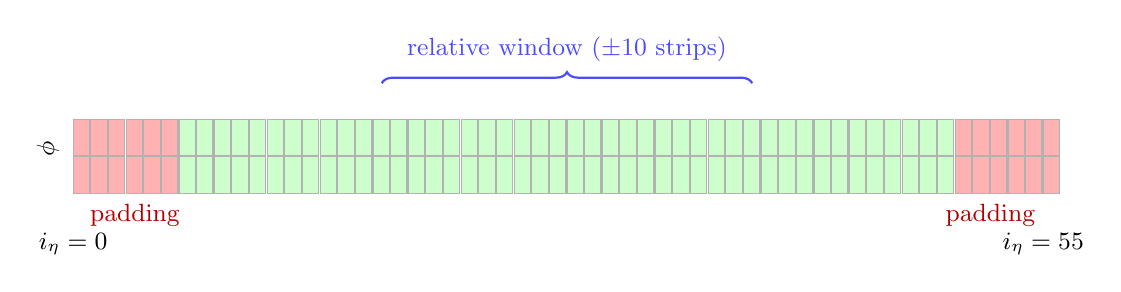
\begin{tikzpicture}[scale=0.8]
    % Draw a 56x2 grid (scaled down) with some padding cells shaded
    \def\cw{0.28}  % cell width
    \def\ch{0.6}   % cell height
    \foreach \i in {0,...,55} {
      \foreach \j in {0,1} {
        % Padding for |i - 28| > 22 (illustrative)
        \pgfmathsetmacro\ispad{ifthenelse(\i < 6 || \i > 49, 1, 0)}
        \ifnum\i<6
          \fill[red!30] (\i*\cw, \j*\ch+0.1) rectangle +(\cw-0.02, \ch-0.02);
        \else\ifnum\i>49
          \fill[red!30] (\i*\cw, \j*\ch+0.1) rectangle +(\cw-0.02, \ch-0.02);
        \else
          \fill[green!20] (\i*\cw, \j*\ch+0.1) rectangle +(\cw-0.02, \ch-0.02);
        \fi\fi
        \draw[gray!60] (\i*\cw, \j*\ch+0.1) rectangle +(\cw-0.02, \ch-0.02);
      }
    }
    % Brace for relative window
    \draw[decorate,decoration={brace,amplitude=4pt},thick,blue!70]
      (17.5*\cw, 1.85) -- (38.5*\cw, 1.85)
      node[midway,above=4pt,font=\small,blue!70] {relative window ($\pm10$ strips)};
    % Labels
    \node[font=\small,red!70!black] at (3.5*\cw, -0.25) {padding};
    \node[font=\small,red!70!black] at (52*\cw, -0.25) {padding};
    \node[font=\small] at (0, -0.7) {$i_\eta = 0$};
    \node[font=\small] at (55*\cw, -0.7) {$i_\eta = 55$};
    \node[font=\small,rotate=90] at (-0.4, 0.8) {$\phi$};
  \end{tikzpicture}
  \caption{Schematic of the Layer-1 absolute $56 \times 2$ cell grid
           (cells in $\eta \times \phi$).  Genuine calorimeter cells
           are shown in green; padding cells (satisfying
           $E = 0 \wedge \eta = 0 \wedge \phi = 0$, \cref{eq:padding})
           are shown in red.  The relative $21 \times 2$ reweighting
           window (blue brace) is centred on the hot-cell position
           after recentering (\cref{sec:method:recentering}).  At
           high $\abseta$ near the barrel--end-cap transition, the
           fraction of padding cells can be large.}
  \label{fig:padding}
\end{figure}

\subsection{Hot-Cell Recentering}
\label{sec:method:recentering}

After excluding padding cells, the relative window used for
reweighting must be centred on the correct cell.  A naive barycentre
(energy-weighted mean position) can be biased by asymmetric energy
deposits, especially in Layer~1 where a single dominant strip carries
most of the signal.  Instead, the pipeline uses \emph{hot-cell
recentering}: the cell carrying the maximum energy deposit within the
absolute grid is identified, and the $21 \times 2$ relative window is
extracted centred on that cell's $\eta$ index.

The algorithm is:
\begin{enumerate}[label=\arabic*.]
  \item Exclude all padding cells (condition \cref{eq:padding}).
  \item Find $k^* = \arg\max_k E_k$ among the remaining cells.
  \item Extract $\eta_\mathrm{rel} = i_\eta(k) - i_\eta(k^*)$ for
        each cell $k$ in the absolute grid.
  \item Retain only cells with $|\eta_\mathrm{rel}| \le 10$ and both
        $\phi$ values.
\end{enumerate}

This procedure ensures that the reweighting maps are always
computed relative to the same physical reference point (the shower
core), regardless of the photon's absolute $\eta$ position within
the cluster window.  \Cref{fig:recentering} illustrates the
before/after comparison.

\begin{figure}[htbp]
  \centering
  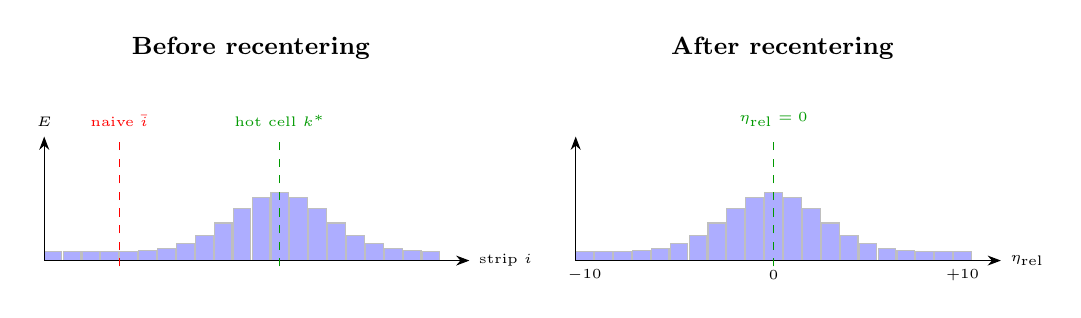
\begin{tikzpicture}[scale=0.75]
    % Before recentering
    \node[font=\small\bfseries] at (3.5,3.6) {Before recentering};
    \foreach \i in {0,...,20} {
      \pgfmathsetmacro\ht{0.15 + 1.0*exp(-0.5*((\i-12)/2.5)^2)}
      \fill[blue!40!white, opacity=0.8]
        (\i*0.32, 0) rectangle ++(0.30, \ht);
      \draw[gray!50] (\i*0.32, 0) rectangle ++(0.30, \ht);
    }
    \draw[-{Stealth}] (0,0) -- (7.2,0) node[right,font=\tiny]{strip $i$};
    \draw[-{Stealth}] (0,0) -- (0,2.1) node[above,font=\tiny]{$E$};
    \draw[dashed,red] (3.5*0.32+0.15, -0.1) -- ++(0,2.2)
      node[above,font=\tiny,red]{naive $\bar{i}$};
    \draw[dashed,green!60!black] (12*0.32+0.15, -0.1) -- ++(0,2.2)
      node[above,font=\tiny,green!60!black]{hot cell $k^*$};

    % After recentering (shifted so hot cell is at centre)
    \node[font=\small\bfseries] at (12.5,3.6) {After recentering};
    \foreach \i in {0,...,20} {
      \pgfmathsetmacro\irel{\i - 10}
      \pgfmathsetmacro\ht{0.15 + 1.0*exp(-0.5*(\irel/2.5)^2)}
      \fill[blue!40!white, opacity=0.8]
        (9.0+\i*0.32, 0) rectangle ++(0.30, \ht);
      \draw[gray!50] (9.0+\i*0.32, 0) rectangle ++(0.30, \ht);
    }
    \draw[-{Stealth}] (9.0,0) -- (16.2,0)
      node[right,font=\tiny]{$\eta_\mathrm{rel}$};
    \draw[-{Stealth}] (9.0,0) -- (9.0,2.1);
    \draw[dashed,green!60!black] (9.0+10*0.32+0.15, -0.1) -- ++(0,2.2)
      node[above,font=\tiny,green!60!black]{$\eta_\mathrm{rel}=0$};
    % Axis labels
    \node[font=\tiny] at (9.0+0*0.32+0.15, -0.25) {$-10$};
    \node[font=\tiny] at (9.0+10*0.32+0.15, -0.25) {$0$};
    \node[font=\tiny] at (9.0+20*0.32+0.15, -0.25) {$+10$};
  \end{tikzpicture}
  \caption{\textit{Left}: The strip-layer energy profile of a
           representative photon before recentering.  The energy
           barycentre (red dashed line) is offset from the hot cell
           (green dashed line) due to asymmetric tails.
           \textit{Right}: After hot-cell recentering, the profile is
           aligned on the hot cell at $\eta_\mathrm{rel} = 0$.
           All 42 cells in the relative grid are used for reweighting.}
  \label{fig:recentering}
\end{figure}

\subsection{The Two-Pass Reweighting Pipeline}
\label{sec:method:twopass}

A single reweighting map (``Method~1'', M1) suffices for Layer~2,
but Layer~1 requires a two-pass procedure because the correction
derived from the integrated sample is not self-consistent when cells
with very low occupancy are involved.  The full pipeline is described
in \cref{fig:pipeline_flowchart}.

\subsubsection{Method~1 (M1): Integrated map}
\label{sec:method:m1}

For each relative cell position $k_r \in [0, 41]$, the reweighting
factor is:
\begin{equation}
  w_{k_r}^\mathrm{M1} =
    \frac{f_{k_r}^\mathrm{data}}{f_{k_r}^\mathrm{MC}}\,,
  \label{eq:m1}
\end{equation}
where
\begin{equation}
  f_{k_r}^X = \frac{\langle E_{k_r} \rangle_X}
                    {\sum_{k'} \langle E_{k'} \rangle_X}
  \label{eq:frac}
\end{equation}
is the mean energy fraction in cell $k_r$ averaged over all photons
in sample $X \in \{\text{data, MC}\}$.  The weight is applied to
the MC event by rescaling all cell energies:
$E_{k_r}^\mathrm{corrected} = w_{k_r}^\mathrm{M1} \cdot E_{k_r}^\mathrm{MC}$.
Total energy is not conserved by this rescaling; a global
renormalisation is applied afterward to restore the total cluster
energy.

\subsubsection{Method~2 (M2): Second-pass map}
\label{sec:method:m2}

M1 assumes that the mean energy fraction is a good proxy for
the per-cell correction.  In Layer~2 this is adequate.  In Layer~1,
however, many cells have very low (or zero) mean energy fractions
(e.g.\ the far-off-centre strips), and the ratio
$f_{k_r}^\mathrm{data} / f_{k_r}^\mathrm{MC}$ can be dominated
by statistical noise or by a small denominator.

Method~2 addresses this by applying M1 corrections first (producing
a partially corrected MC sample) and then deriving a residual
correction from the difference between data and the M1-corrected MC:
\begin{align}
  w_{k_r}^\mathrm{M2} &=
    w_{k_r}^\mathrm{M1} \cdot
    \frac{f_{k_r}^\mathrm{data}}{f_{k_r}^{\mathrm{MC, M1}}}\,,
  \label{eq:m2}
\end{align}
where $f_{k_r}^{\mathrm{MC, M1}}$ is the mean energy fraction of
the M1-corrected MC.  The final M2 weight is thus a product of the
two successive corrections.  Cells for which
$f_{k_r}^{\mathrm{MC, M1}} < f_\mathrm{min}$ (with safety threshold
$f_\mathrm{min} = 0.002$ in the Layer-1 configuration,
\texttt{kMinFracForM2\_L1}) are left unchanged at the M1 value
to avoid division by zero or unphysical amplification.

\subsubsection{Flowchart}
\label{sec:method:flowchart}

\begin{figure}[htbp]
  \centering
  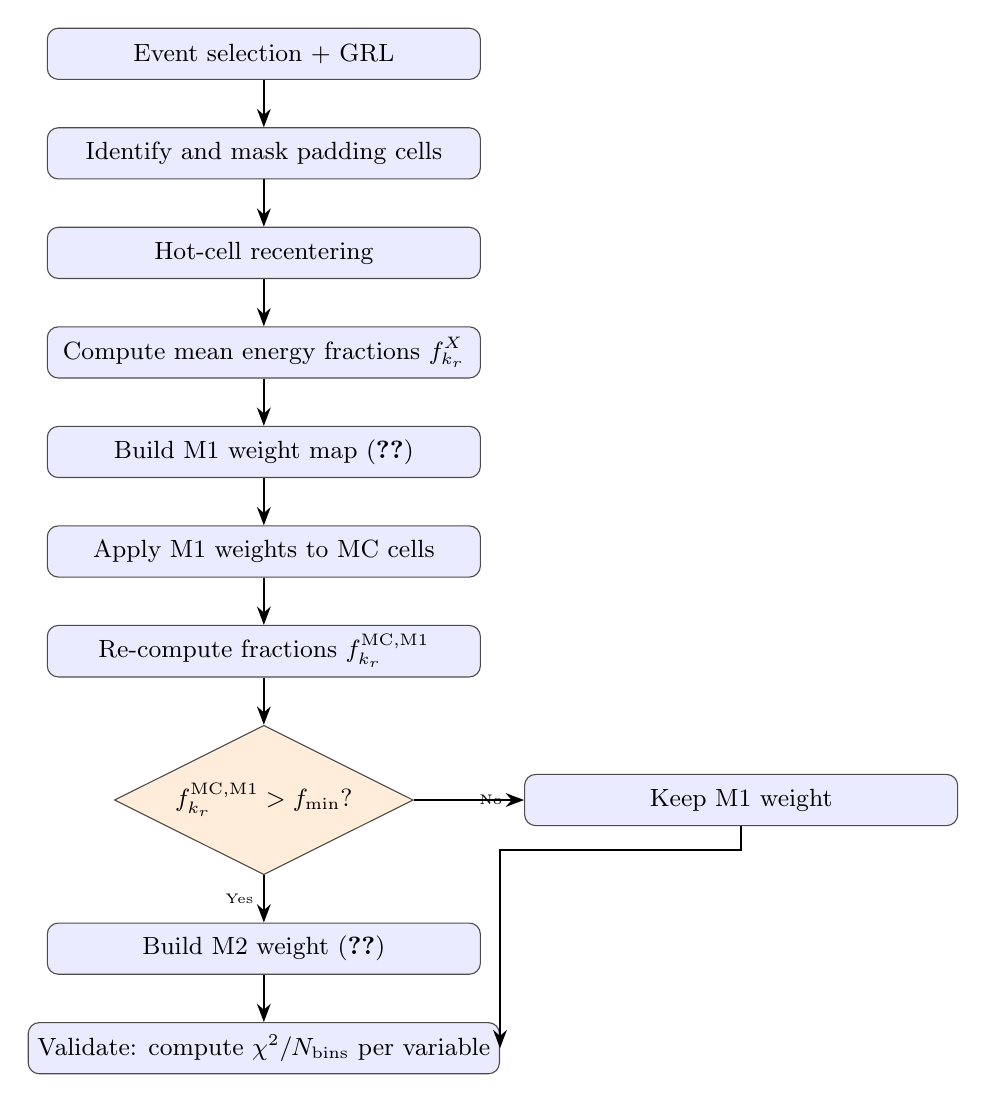
\begin{tikzpicture}[
    node distance=0.6cm and 1.2cm,
    box/.style={rectangle,rounded corners,draw=black!70,
                fill=blue!8,minimum width=5.5cm,
                minimum height=0.65cm,align=center,font=\small},
    decision/.style={diamond,draw=black!70,fill=orange!15,
                     minimum width=2.5cm,minimum height=0.7cm,
                     align=center,font=\small,aspect=2},
    arrow/.style={-{Stealth},thick},
    ]
    \node[box] (sel) {Event selection + GRL};
    \node[box,below=of sel] (pad) {Identify and mask padding cells};
    \node[box,below=of pad] (rec) {Hot-cell recentering};
    \node[box,below=of rec] (frac) {Compute mean energy fractions $f_{k_r}^X$};
    \node[box,below=of frac] (m1)  {Build M1 weight map (\cref{eq:m1})};
    \node[box,below=of m1]   (app) {Apply M1 weights to MC cells};
    \node[box,below=of app]  (m2frac) {Re-compute fractions $f_{k_r}^{\mathrm{MC,M1}}$};
    \node[decision,below=of m2frac] (thresh)
      {$f_{k_r}^{\mathrm{MC,M1}} > f_\mathrm{min}$?};
    \node[box,right=1.4cm of thresh] (skip) {Keep M1 weight};
    \node[box,below=0.6cm of thresh] (m2)  {Build M2 weight (\cref{eq:m2})};
    \node[box,below=of m2]   (val)  {Validate: compute $\chisq$ per variable};

    \draw[arrow] (sel) -- (pad);
    \draw[arrow] (pad) -- (rec);
    \draw[arrow] (rec) -- (frac);
    \draw[arrow] (frac) -- (m1);
    \draw[arrow] (m1)  -- (app);
    \draw[arrow] (app) -- (m2frac);
    \draw[arrow] (m2frac) -- (thresh);
    \draw[arrow] (thresh) -- node[right,font=\tiny]{No} (skip);
    \draw[arrow] (thresh) -- node[left,font=\tiny]{Yes} (m2);
    \draw[arrow] (m2)  -- (val);
    \draw[arrow] (skip.south) -- ++(0,-0.3) -| (val.east);
  \end{tikzpicture}
  \caption{Flowchart of the two-pass cell-level reweighting pipeline.
           Both Method~1 (M1) and Method~2 (M2) maps are produced;
           M2 adds a residual correction on top of M1 for cells where
           the M1-corrected fraction exceeds the safety threshold.}
  \label{fig:pipeline_flowchart}
\end{figure}

\subsection{Validation Metric: \texorpdfstring{$\chisq$}{chi2/nbins}}
\label{sec:method:validation}

Correction quality is quantified by comparing the data and MC
distributions of each shower-shape variable using
\begin{equation}
  \chisq = \frac{1}{N_\mathrm{bins}}
    \sum_{i=1}^{N_\mathrm{bins}}
    \frac{(n_i^\mathrm{data} - n_i^\mathrm{MC})^2}
         {\sigma_i^2}\,,
  \label{eq:chi2}
\end{equation}
where $n_i^X$ is the bin content normalised to unit area,
$\sigma_i^2 = (\sigma_i^\mathrm{data})^2 + (\sigma_i^\mathrm{MC})^2$
is the combined statistical uncertainty, and $N_\mathrm{bins}$ is the
number of bins.  A value $\chisq \to 0$ indicates perfect agreement;
$\chisq = 1$ corresponds to agreement within one standard deviation
per bin on average.

The comparison is performed for each variable in each
correction scenario: (i)~uncorrected MC (\textbf{MC}), (ii)~M1-corrected
MC, (iii)~M2-corrected MC, and (iv)~fudge-factor corrected MC
(\textbf{Fudged}).

\subsection{Real Data Plots}
\label{sec:method:realplots}

\Cref{fig:cell_data_l1,fig:cell_shift_l1}
show representative cell-level plots produced by the pipeline for
the $\eta \in [0.0, 0.2)$ bin of the unconverted llgamma sample.

\begin{figure}[htbp]
  \centering
  \includegraphics[width=0.62\textwidth]{cell_data.pdf}
  \caption{Mean energy fraction per cell in the $21\times2$ Layer-1
           relative grid for data photons (unconverted,
           $\abseta \in [0.0, 0.2)$, llgamma sample).  The dominant
           energy is concentrated in the two central strips
           ($\eta_\mathrm{rel} = 0$), with rapidly falling tails.}
  \label{fig:cell_data_l1}
\end{figure}

\begin{figure}[htbp]
  \centering
  \includegraphics[width=0.62\textwidth]{cell_shift.pdf}
  \caption{Relative shift map $(f^\mathrm{data} - f^\mathrm{MC})/f^\mathrm{MC}$
           per cell for Layer~1 (unconverted, $\abseta \in [0.0, 0.2)$).
           Positive (red) cells are under-estimated in MC; negative
           (blue) cells are over-estimated.  The central strips
           show a systematic deficit in MC relative to data.}
  \label{fig:cell_shift_l1}
\end{figure}


% ============================================================
\section{Why Layer~1 Is Harder Than Layer~2}
\label{sec:layer1}
% ============================================================

The cell-level reweighting achieves excellent results in Layer~2 but
substantially more modest improvements in Layer~1.  This section
provides a detailed physical and statistical analysis of why
Layer~1 presents unique difficulties, supported by the quantitative
$\chisq$ comparisons from the analysis runs.

\subsection{Physical Reasons}
\label{sec:layer1:physical}

\subsubsection{Extreme Aspect Ratio}

As detailed in \cref{sec:atlas:layer1}, Layer-1 strip cells have
$\Delta\eta / \Delta\phi \approx 0.003125 / 0.1 \approx 1/32$.
The reweighting grid is therefore $21 \times 2$ (not $7 \times 11$
as in Layer~2), and both $\phi$ slots for a given $\eta$ index
must be treated as one effective measurement.  The two-cell $\phi$
dimension provides essentially no $\phi$-resolved information,
making it impossible to study the azimuthal shower profile in L1.

\subsubsection{Low Signal-to-Noise per Cell}

The energy deposited in an individual L1 strip cell by a
$\pt \sim 40\,\mathrm{GeV}$ photon is typically
$\mathcal{O}(50$--$200\,\mathrm{MeV})$, comparable to the
electronic noise ($\sim$$50\,\mathrm{MeV}$ per cell).  In contrast,
the signal per Layer-2 cell is $\mathcal{O}(1$--$5\,\mathrm{GeV})$,
giving a signal-to-noise ratio $\sim$20--100$\times$ larger.
Low-SNR cells are dominated by noise fluctuations, making the
mean energy fraction $f_{k_r}$ measured in finite data samples noisy
and biased, particularly in the off-centre strips.

\subsubsection{Sensitivity to Shower Substructure Variables}

The key Layer-1 discrimination variables ($\dE$, $\Eratio$, $\wstot$)
depend critically on the positions and amplitudes of local
\emph{maxima} and \emph{minima} in the strip profile — features that
require accurate modelling of the profile shape over a dynamic range
of several orders of magnitude.  A mean energy fraction map (the
basis of M1/M2) captures the average profile shape but is insensitive
to the \emph{distribution} of profiles across events.  In particular:
\begin{itemize}
  \item $\Eratio$ depends on the ratio of the two largest strip maxima.
        If the second maximum is in a cell that, on average, has low
        energy ($f_{k_r} \approx 0$), the M1 weight for that cell may be
        ill-defined and the ratio is not corrected.
  \item $\dE$ depends on the energy difference between the second
        maximum and the adjacent minimum.  Noise fills in the minimum,
        inflating $\dE$ in a way not captured by mean-fraction corrections.
  \item $\wstot$ uses a 40-strip window in which most strips are noise.
        The variance of noise-dominated tails is sensitive to the noise
        model, not the shower model.
\end{itemize}

\subsubsection{Hot-Strip Jitter}

The hot-cell (maximum-energy cell) used for recentering has
quantised $\eta$ values.  In Layer~2, where cells are
$\Delta\eta = 0.025$ wide, the shift between events in the
maximum's $\eta$ bin is small relative to the shower width.
In Layer~1, where cells are $\Delta\eta = 0.003125$ wide, a single
strip offset corresponds to only $0.3\%$ of the $\Delta\eta_{\mathrm{Moli\grave{e}re}}$
lateral scale.  This means that \emph{event-to-event jitter in the
hot-strip identification} introduces a stochastic misalignment in the
recentered grid that slightly smears the mean energy fraction maps.

\subsubsection{Crack Region and Transition Effects}

Near $\abseta \approx 1.37$ (the barrel--end-cap transition), the
Layer-1 cell granularity changes abruptly (see \cref{tab:granularity})
and the fraction of padding cells increases.  Events near the crack
have more missing cells, noisier barycentre estimates, and partially
populated relative grids, all of which degrade the correction quality.
Even after the ``eta\_loose'' selection ($\abseta < 2.4$ excluding
the crack $[1.37, 1.52]$), the photons closest to the crack
boundaries have a worse reweighting performance.

\subsection{Quantitative $\chisq$ Comparison}
\label{sec:layer1:chi2}

\Cref{tab:chi2_l1,tab:chi2_l2} present the $\chisq$ values
(unconverted llgamma, $\eta$ bin $[0.0, 0.2)$) for all correction
scenarios: uncorrected MC (MC), M1-corrected, M2-corrected, and
fudge-factor corrected (Fudged).

\begin{table}[htbp]
  \centering
  \caption{$\chisq$ for Layer-1 shower-shape variables
           (unconverted photons, $\abseta \in [0.0, 0.2)$, llgamma
           sample).  Values $\lesssim 0.001$ indicate excellent
           agreement.  Bold indicates the best non-fudge scenario.}
  \label{tab:chi2_l1}
  \begin{tabular}{lcccc}
    \toprule
    Variable & MC & M1 & M2 & Fudged \\
    \midrule
    $\wetaone$ & 0.0071 & 0.0123 & \textbf{0.0059} & 0.0005 \\
    $\wstot$   & 0.0029 & 0.0538 & 0.0446          & \textbf{0.0005} \\
    $\fside$   & 0.0043 & 0.0140 & 0.0129          & \textbf{0.0004} \\
    $\dE$      & 0.0009 & 0.0076 & 0.0083          & \textbf{0.0007} \\
    $\Eratio$  & 0.0004 & 0.0526 & 0.0553          & \textbf{0.0004} \\
    \bottomrule
  \end{tabular}
\end{table}

\begin{table}[htbp]
  \centering
  \caption{$\chisq$ for Layer-2 shower-shape variables
           (unconverted photons, $\abseta \in [0.0, 0.2)$, llgamma
           sample).  M2 achieves near-fudge performance for all
           three variables.}
  \label{tab:chi2_l2}
  \begin{tabular}{lcccc}
    \toprule
    Variable & MC & M1 & M2 & Fudged \\
    \midrule
    $\Reta$  & 0.0015 & 0.0006 & \textbf{0.0005} & 0.0005 \\
    $\Rphi$  & 0.0007 & 0.0011 & \textbf{0.0006} & 0.0005 \\
    $\weta$  & 0.0076 & 0.0007 & \textbf{0.0005} & 0.0005 \\
    \bottomrule
  \end{tabular}
\end{table}

The contrast is striking.  For Layer~2, M2 achieves $\chisq \le 0.0006$
for all variables, matching or approaching the fudge-factor level.
For Layer~1, M2 corrects $\wetaone$ from 0.0071 to 0.0059 — a
partial improvement — but actually \emph{worsens} $\wstot$
(0.0029 $\to$ 0.0446), $\dE$ (0.0009 $\to$ 0.0083), and
$\Eratio$ (0.0004 $\to$ 0.0553).  These variables are all sensitive
to the substructure features discussed in \cref{sec:layer1:physical}
(local maxima/minima, noise-dominated tails) that mean-fraction maps
cannot correctly reproduce.

\paragraph{Interpretation.}
The M1 and M2 maps shift energy toward the central strips and away
from the wings, which correctly improves $\wetaone$ but simultaneously
distorts the shape of the secondary-peak region.  The substructure
variables ($\Eratio$, $\dE$, $\wstot$) depend on this shape, so they
deteriorate.  This is a fundamental limitation of the mean-fraction
approach for variables that are sensitive to the \emph{shape of the
distribution} rather than its mean.

\begin{figure}[htbp]
  \centering
  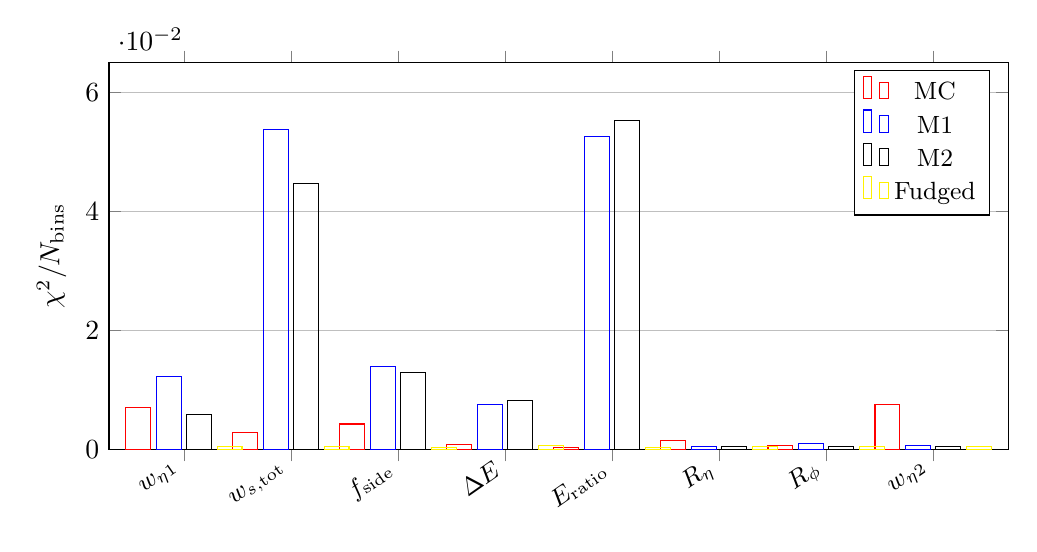
\begin{tikzpicture}
    % Bar chart comparing chi2 across layers
    \begin{axis}[
      ybar, bar width=9pt,
      symbolic x coords={$\wetaone$,$\wstot$,$\fside$,$\dE$,$\Eratio$,
                          $\Reta$,$\Rphi$,$\weta$},
      xtick=data,
      x tick label style={rotate=35,anchor=east,font=\small},
      ylabel={$\chi^2/N_\mathrm{bins}$},
      ymin=0, ymax=0.065,
      width=13cm, height=6.5cm,
      legend style={at={(0.98,0.98)},anchor=north east,font=\small},
      ymajorgrids=true,
      cycle list name=color list,
    ]
    \addplot coordinates {
      ($\wetaone$,0.0071)($\wstot$,0.0029)($\fside$,0.0043)
      ($\dE$,0.0009)($\Eratio$,0.0004)
      ($\Reta$,0.0015)($\Rphi$,0.0007)($\weta$,0.0076)
    };
    \addplot coordinates {
      ($\wetaone$,0.0123)($\wstot$,0.0538)($\fside$,0.0140)
      ($\dE$,0.0076)($\Eratio$,0.0526)
      ($\Reta$,0.0006)($\Rphi$,0.0011)($\weta$,0.0007)
    };
    \addplot coordinates {
      ($\wetaone$,0.0059)($\wstot$,0.0446)($\fside$,0.0129)
      ($\dE$,0.0083)($\Eratio$,0.0553)
      ($\Reta$,0.0005)($\Rphi$,0.0006)($\weta$,0.0005)
    };
    \addplot coordinates {
      ($\wetaone$,0.0005)($\wstot$,0.0005)($\fside$,0.0004)
      ($\dE$,0.0007)($\Eratio$,0.0004)
      ($\Reta$,0.0005)($\Rphi$,0.0005)($\weta$,0.0005)
    };
    \legend{MC, M1, M2, Fudged}
    \end{axis}
  \end{tikzpicture}
  \caption{$\chisq$ comparison across all shower-shape variables
           and correction scenarios.  Layer-1 variables are on the
           left (5 bars per group) and Layer-2 variables on the right
           (3 bars per group).  Note that M1/M2 dramatically improve
           Layer-2 variables but worsen several Layer-1 substructure
           variables ($\wstot$, $\Eratio$) relative to uncorrected MC.}
  \label{fig:chi2_comparison}
\end{figure}


% ============================================================
\section{Binning Optimisation}
\label{sec:binning}
% ============================================================

\subsection{Current Binning Scheme}
\label{sec:binning:current}

The current correction maps are derived in the following bins:
\begin{itemize}
  \item \textbf{$|\eta|$ bin}: Three ``eta'' categories — \texttt{eta\_loose}
        ($\abseta < 2.4$ excluding crack $[1.37, 1.52]$),
        \texttt{eta\_barrel} ($\abseta < 1.37$), and
        \texttt{eta\_endcap} ($1.52 < \abseta < 2.4$).
  \item \textbf{Conversion status}: Unconverted and converted
        sub-samples treated independently.
  \item \textbf{Data sample}: Derived separately from
        $Z \to ee\gamma$ and $Z \to \mu\mu\gamma$ and then combined.
\end{itemize}

No $p_\mathrm{T}$ binning or pile-up ($\avgmu$) binning is applied in
the baseline run.  This is a significant simplification: shower shapes
have a mild but non-negligible $p_\mathrm{T}$ dependence (the shower
maximum depth $t_\mathrm{max} \propto \ln p_\mathrm{T}$,
\cref{eq:shower:long}), and the pile-up contribution to cell energies
grows with $\avgmu$.

\subsection{Proposed Improvements}
\label{sec:binning:proposed}

\subsubsection{Finer $|\eta|$ Binning}

The LAr granularity and the material budget both vary strongly with
$\eta$ (see \cref{tab:granularity}).  The crack region
$[1.37, 1.52]$ is currently excluded; the immediately adjacent bins
$[1.2, 1.37]$ and $[1.52, 1.6]$ likely have residual transition
effects that are averaged away in the current coarse $\eta$
categorisation.  A finer binning with $\Delta\eta \approx 0.1$--$0.2$
across the full range would resolve these gradients, at the cost of
reduced per-bin statistics.

The barrel region $\abseta < 0.6$ is particularly uniform and allows
coarser binning; the end-cap region $\abseta > 2.0$ has rapidly
changing granularity and would benefit from finer binning.

\subsubsection{$p_\mathrm{T}$ Binning}

The longitudinal shower development depends logarithmically on the
photon energy: $t_\mathrm{max} \propto \ln(E/E_c)$.  At low
$p_\mathrm{T} \sim 15\,\mathrm{GeV}$ the shower maximum lies closer
to the PS/L1 boundary; at high $p_\mathrm{T} \sim 200\,\mathrm{GeV}$
it shifts deeper into L2.  The \emph{relative} energy fraction in
each cell therefore has a genuine $p_\mathrm{T}$ dependence that
cannot be captured by a single map.

A coarse $p_\mathrm{T}$ binning in three bins
(e.g.\ $[15, 30]$, $[30, 60]$, $[60, 200]\,\mathrm{GeV}$) would
improve the correction accuracy without unduly fragmenting the
control sample statistics.  The $Z \to \ell\ell\gamma$ sample has
a kinematic constraint: the photon $p_\mathrm{T}$ is bounded by
$m_{Z}/2 \approx 46\,\mathrm{GeV}$, so the high-$p_\mathrm{T}$
bin will have lower statistics and may need to be supplemented
with other control processes (e.g.\ $Z + \gamma$ or isolated photons
from $W + \gamma$).

\subsubsection{Pile-up ($\avgmu$) Binning}

Pile-up contributes a per-cell energy offset with a distribution
that depends on the local pile-up density.  In Layer~1, where the
cell noise is already comparable to the signal, the pile-up
contribution can appreciably change the mean fraction $f_{k_r}$.
Run-3 data at $\avgmu \sim 50$--$70$ may require pile-up-specific
correction maps.

A binning in $\avgmu$ into low ($< 30$), medium ($30$--$50$), and
high ($> 50$) categories is feasible with the full Run-3 dataset
but is borderline feasible with Run-2 statistics alone.  Alternatively,
a continuous pile-up subtraction could be applied to each cell before
building the correction maps.

\subsubsection{Sub-Cell $\eta$ Position}

Within a given strip cell, the photon impact position (in fractional
strip units $\eta_\mathrm{cell} = (\eta_\mathrm{photon} - \eta_\mathrm{cell\,centre})/\Delta\eta$)
affects the energy sharing between adjacent strips.  Correcting for this
``within-cell'' position would require an additional continuous variable
in the correction map, moving toward a fully differential approach
that naturally motivates normalising flow methods (\cref{sec:alternatives:nf}).

\subsubsection{Statistics Constraints}

\Cref{tab:stats_budget} shows the approximate per-bin event count
for the current scheme and the proposed extensions.  With Run-2 data
($\sim 140\,\mathrm{fb}^{-1}$), $p_\mathrm{T}$ and $\avgmu$ binning
become feasible at the level of $\mathcal{O}(10^3)$ events per bin
cell, which is sufficient for the 42-cell L1 maps.  For Run-3 the
statistics improve by a factor of $\sim$3.

\begin{table}[htbp]
  \centering
  \caption{Approximate event counts in the control sample for the
           current binning scheme and proposed extensions (Run-2,
           llgamma sample, unconverted).  ``Sufficient'' means
           $\gtrsim 500$ events per bin cell.}
  \label{tab:stats_budget}
  \begin{tabular}{lccc}
    \toprule
    Binning scheme & $N_\eta$ & $N_{p_\mathrm{T}}$ & Approximate events/bin \\
    \midrule
    Current (eta\_loose) & 1 & 1 & $\sim 200{,}000$ \\
    Finer $\eta$ ($\Delta\eta=0.2$) & 12 & 1 & $\sim 16{,}000$ \\
    $\eta + p_\mathrm{T}$ & 12 & 3 & $\sim 5{,}000$ \\
    $\eta + p_\mathrm{T} + \avgmu$ & 12 & 3 & $\sim 1{,}500$ \\
    \bottomrule
  \end{tabular}
\end{table}

% ============================================================
\section{Alternative Correction Methods}
\label{sec:alternatives}
% ============================================================

The results in \cref{sec:layer1:chi2} show that the mean-fraction
approach (M1/M2) fails for Layer-1 substructure variables.  This
motivates a survey of alternative methodologies that could overcome
the limitations identified in \cref{sec:layer1:physical}.  All
methods described below have been demonstrated in high-energy physics
or adjacent fields; none are currently deployed in ATLAS for
shower-shape corrections.

\subsection{Normalising Flows}
\label{sec:alternatives:nf}

A \emph{normalising flow}~\cite{Papamakarios:2021,NSF:2019,MAF:2017}
is a class of invertible neural network that learns a bijective
mapping $T: \mathcal{X} \to \mathcal{Z}$ between a target
distribution $p_X(x)$ and a simple base distribution
$p_Z(z)$ (typically a standard Gaussian).  The density is
computed exactly via the change-of-variables formula:
\begin{equation}
  \ln p_X(x) = \ln p_Z(T(x)) + \ln\left|
    \det \frac{\partial T(x)}{\partial x}\right|\,.
  \label{eq:nf:density}
\end{equation}
Because the mapping is invertible, one can generate samples from
$p_X$ by sampling $z \sim p_Z$ and applying $T^{-1}(z)$.

\subsubsection{Architecture}

Modern normalising flows for high-dimensional data use
\emph{coupling layers}~\cite{RealNVP:2017}: the input vector $x$ is
split into two halves $(x_A, x_B)$; the first half is passed
unchanged and the second half is transformed by an invertible
function whose parameters are predicted by a neural network
applied to $x_A$:
\begin{align}
  z_A &= x_A \\
  z_B &= f_\theta(x_B;\, s(x_A),\, t(x_A))\,,
  \label{eq:nf:coupling}
\end{align}
where $s$ and $t$ are scale and translation networks (the ``affine
coupling'' of RealNVP).  The Jacobian of this transformation is
triangular, making \cref{eq:nf:density} cheap to evaluate.

For the shower-shape correction problem, one would:
\begin{enumerate}[label=\arabic*.]
  \item Train a flow on the 42-dimensional cell-energy fraction
        vector from \emph{data} photons.
  \item Transform each MC event to the latent space, resample or
        transport it toward the data density, and map back.
\end{enumerate}
This approach operates on the full joint distribution of all 42 cells
simultaneously, correctly propagating correlations.

\paragraph{Relevance to Layer~1.}
Normalising flows can model multi-modal distributions (e.g.\ the
bimodal strip profile of $\pi^0$ events) that mean-fraction maps
cannot represent.  They are also naturally differentiable, enabling
gradient-based uncertainty propagation.

\subsubsection{Practical Considerations}

Training a normalising flow on 42-dimensional data requires
$\mathcal{O}(10^5$--$10^6)$ events, which is feasible with Run-3
statistics.  The main technical challenges are:
\begin{itemize}
  \item \textbf{Sparsity}: Many cells have near-zero energy fractions.
        A logit-space or normalised-energy-fraction parameterisation
        should be used to avoid boundary effects.
  \item \textbf{Conditioning}: The flow should be conditioned on
        $(\eta, p_\mathrm{T}, \avgmu, \text{conversion status})$
        to learn the correct distribution in each kinematic regime.
  \item \textbf{Evaluation cost}: Inference is a forward pass through
        the network, adding $\mathcal{O}(\mathrm{ms})$ per event —
        acceptable for offline corrections.
\end{itemize}

\subsection{Classifier-Based Reweighting (CARL)}
\label{sec:alternatives:carl}

The CARL (Classifier-Aided Ratio Learning) approach~\cite{CARL:2016}
learns the likelihood ratio
$r(x) = p_\mathrm{data}(x) / p_\mathrm{MC}(x)$
by training a classifier $f_\theta(x)$ to distinguish data
from MC.  Under the optimal Bayes classifier, the probability
ratio is:
\begin{equation}
  r(x) = \frac{p_\mathrm{data}(x)}{p_\mathrm{MC}(x)}
         = \frac{f_\theta(x)}{1 - f_\theta(x)}\,,
  \label{eq:carl}
\end{equation}
where the classifier is trained with balanced class weights.
Each MC event is then assigned weight $w = r(x)$ to reweight it
toward the data distribution.

\paragraph{Application to cell-level corrections.}
The CARL weight can be computed as a function of the full
42-dimensional cell vector (or of the 112-cell absolute grid with
padding mask), allowing simultaneous correction of all
cells~\cite{Rizvi:2023}.  Because the classifier is a discriminative
model, it does not need to model the absolute density — only the
ratio — which is generally easier to learn and requires less data.

\paragraph{Limitations.}
\begin{itemize}
  \item The classifier output is an event-level weight, not a cell-level
        transformation.  It can improve agreement in high-level
        distributions but does not provide cell-by-cell correction maps
        for diagnostic purposes.
  \item High-dimensional input classifiers require careful regularisation
        to avoid overfitting on statistical fluctuations in finite
        data/MC samples.
\end{itemize}

\subsection{Optimal Transport}
\label{sec:alternatives:ot}

Optimal transport (OT)~\cite{Villani:2009,Peyre:2019} provides a
principled mathematical framework for transforming one
distribution $p_\mathrm{MC}$ into another $p_\mathrm{data}$.
The \emph{Wasserstein-2} ($W_2$) barycenter map is the unique
measure-preserving transport that minimises the expected squared
displacement:
\begin{equation}
  T^* = \arg\min_T \int \|x - T(x)\|^2 \, p_\mathrm{MC}(x)\,
        \mathrm{d}x\,,
  \quad
  T_\# p_\mathrm{MC} = p_\mathrm{data}\,.
  \label{eq:ot:w2}
\end{equation}
In one dimension, $T^*$ is the quantile transform $T^*(x) =
F_\mathrm{data}^{-1}(F_\mathrm{MC}(x))$.  In high dimensions,
the OT map must be approximated numerically.

\paragraph{Energy mover's distance (EMD).}
The EMD~\cite{Komiske:2019} is a special case of the Wasserstein
distance applied to energy flow within a calorimeter event,
treating cell energies as a discrete measure.  An OT-based correction
would find the minimum-cost transport of the MC cell energy
distribution to match the data distribution.  This is physically
motivated: it transforms as few cells as possible (in an energy-cost
sense) to achieve agreement.

\paragraph{Practical implementation.}
Scalable OT algorithms such as Sinkhorn regularisation~\cite{Cuturi:2013}
can handle 42-dimensional distributions with $\mathcal{O}(10^4)$
events per iteration.  Neural OT methods (e.g.\ input-convex neural
networks for the Brenier potential) have been demonstrated for
calorimeter applications~\cite{NachmanShih:2020}.

\subsection{Diffusion Models}
\label{sec:alternatives:diffusion}

Diffusion models~\cite{CaloScore:2022,Butter:2022} learn to reverse a
gradual noising process: a forward Markov chain adds Gaussian noise
to the data over $T$ steps, and a neural network learns to denoise
each step.  At inference, clean samples are generated by
iteratively denoising pure Gaussian noise.

For shower-shape correction, a \emph{conditional} diffusion model
could be trained to generate corrected MC events given the
uncorrected MC input, conditioned on the kinematic variables.
This is analogous to image-to-image translation in computer vision,
where diffusion models currently achieve state-of-the-art performance.

Diffusion models have been applied to calorimeter simulation
(CaloScore, \cite{CaloScore:2022}) but not yet to
data/MC corrections.  The main challenge is that the model must
learn a transport (MC $\to$ data) rather than a generation
(noise $\to$ data) task, which requires careful design of the
conditioning architecture.

\subsection{Method Comparison}
\label{sec:alternatives:comparison}

\Cref{tab:method_comparison} summarises the key properties of each
approach.

\begin{table}[htbp]
  \centering
  \caption{Comparison of alternative correction methods for
           cell-level shower-shape reweighting.}
  \label{tab:method_comparison}
  \small
  \begin{tabular}{lp{2.8cm}p{2.8cm}p{3.0cm}}
    \toprule
    Method & Strengths & Weaknesses & Status in HEP \\
    \midrule
    Mean-fraction (M1/M2) &
      Fast; interpretable; no training &
      Cannot correct distribution shape; fails for substructure vars &
      Currently deployed (this work) \\[4pt]
    Fudge factors &
      Simple; reliable for means &
      Variable-by-variable; no cell info &
      ATLAS standard \\[4pt]
    Normalising flow &
      Full joint distribution; invertible; generative &
      Requires large dataset; complex training; sparsity handling &
      CaloGAN~\cite{CaloGAN:2018}, FastCaloFlow \\[4pt]
    CARL &
      Learns ratio directly; flexible classifier &
      Event weight only; overfitting risk &
      Demonstrated in EFT~\cite{CARL:2016,Rizvi:2023} \\[4pt]
    Optimal transport &
      Physically motivated; minimal displacement &
      Computationally expensive in high-$d$ &
      EMD~\cite{Komiske:2019}, OmniFold~\cite{OmniFold:2020} \\[4pt]
    Diffusion model &
      High fidelity; handles complex topology &
      Slow inference; requires large training set &
      CaloScore~\cite{CaloScore:2022} \\
    \bottomrule
  \end{tabular}
\end{table}


% ============================================================
\section{Conclusions}
\label{sec:conclusions}
% ============================================================

This report has provided a self-contained treatment of the
cell-level shower-shape reweighting methodology developed for the
ATLAS LAr EM calorimeter, covering the detector physics, shower-shape
variable definitions, the origin of data/MC discrepancies, the full
technical pipeline (including padding identification, hot-cell
recentering, and the two-pass M1/M2 correction scheme), and a
detailed analysis of why Layer~1 presents greater challenges
than Layer~2.  The main findings are:

\begin{enumerate}[label=\arabic*.]
  \item \textbf{Layer~2 corrections work well.}
        The M2 correction achieves $\chisq \le 0.0006$ for all three
        Layer-2 variables ($\Reta$, $\Rphi$, $\weta$), reaching or
        approaching fudge-factor-level agreement (0.0005).  The
        mean-fraction approach is adequate for Layer~2 because the
        variables depend only on the mean profile shape, which the
        maps capture correctly.

  \item \textbf{Layer~1 corrections are partial and must be used selectively.}
        M2 improves $\wetaone$ from $\chisq = 0.0071$ to 0.0059 but
        significantly worsens $\wstot$ (0.0029 $\to$ 0.0446),
        $\dE$ (0.0009 $\to$ 0.0083), and $\Eratio$ (0.0004 $\to$ 0.0553).
        Mean-fraction maps cannot correct variables that depend on
        local maxima/minima and the tails of the strip-energy
        distribution.

  \item \textbf{The root cause is structural.}
        The failure for $\Eratio$ and $\dE$ is not a bug but a
        fundamental limitation of the mean-fraction approach: it
        corrects the mean cell occupancy but not the event-by-event
        distribution shape.  This is exacerbated by the low SNR,
        extreme aspect ratio, and substructure sensitivity of L1.

  \item \textbf{Four concrete actions for Layer~1.}
        Based on the analysis in \cref{sec:binning,sec:alternatives}:
        \begin{enumerate}[label=(\alph*)]
          \item Implement finer $|\eta|$ binning ($\Delta\eta \approx 0.2$)
                to resolve gradient effects near the barrel--end-cap
                transition.
          \item Add $p_\mathrm{T}$ binning (3 coarse bins) to account
                for the energy-dependent shower depth.
          \item Restrict M1/M2 corrections to $\wetaone$ only (or at
                most $\fside$, which shows modest improvement), and
                leave $\wstot$, $\dE$, $\Eratio$ uncorrected or fudge
                them separately.
          \item Investigate normalising flows or CARL as the next step
                for a full-distribution correction of $\Eratio$.
        \end{enumerate}

  \item \textbf{Cell-level corrections are the right long-term strategy.}
        Despite the current limitations in Layer~1, cell-level
        corrections are the only approach that can simultaneously
        improve the modelling of ML classifiers operating at the cell
        level (e.g.\ for the ATLAS CP structure measurement) and of
        traditional high-level shower-shape variables.
\end{enumerate}

\paragraph{Recommended next step.}
The highest-priority next step is a normalising flow trained on the
42-cell Layer-1 vector conditioned on $(\abseta, p_\mathrm{T})$,
demonstrated first in the $\abseta < 0.6$ barrel region where the
geometry is most uniform and statistics are highest.  A comparison
with the CARL approach on the same data would establish the
optimal framework for Run-3 corrections.

% ============================================================
\appendix
% ============================================================

\section{Full Calorimeter Granularity Table}
\label{app:granularity}

\Cref{tab:granularity_full} extends \cref{tab:granularity} with
complete coverage of all $\eta$ regions and all calorimeter layers
relevant to EM shower measurement.

\begin{longtable}{lllccc}
  \caption{Complete LAr EM calorimeter cell granularity
           $\Delta\eta \times \Delta\phi$ in all sampling layers
           and $\eta$ regions~\cite{ATLAS:2008,LArTDR:1996}.}
  \label{tab:granularity_full}\\
  \toprule
  Layer & $|\eta|$ range & $\Delta\eta \times \Delta\phi$ &
  $N_\phi$ & Depth [$X_0$] & Primary use \\
  \midrule
  \endfirsthead
  \multicolumn{6}{c}{\small\itshape (continued)}\\
  \toprule
  Layer & $|\eta|$ range & $\Delta\eta \times \Delta\phi$ &
  $N_\phi$ & Depth [$X_0$] & Primary use \\
  \midrule
  \endhead
  \bottomrule
  \endfoot
  PS & $[0.0, 1.52]$ & $0.025\times0.1$ & 64 & 1.5 & Upstream loss \\
  PS & $[1.5, 1.8]$ & $0.025\times0.1$ & 64 & 1.5 & Upstream loss \\
  \midrule
  L1 barrel & $[0.0, 1.40]$ & $0.003125\times0.1$ & 64 & 4.3 & $\pi^0$ rejection \\
  L1 barrel & $[1.40, 1.475]$ & $0.025\times0.025$ & 256 & 4.3 & Transition \\
  L1 end-cap & $[1.5, 1.8]$ & $0.025\times0.1$ & 64 & 4.3 & EM shower \\
  L1 end-cap & $[1.8, 2.0]$ & $0.0125\times0.1$ & 64 & 4.3 & EM shower \\
  L1 end-cap & $[2.0, 2.4]$ & $0.00625\times0.1$ & 64 & 4.3 & $\pi^0$ rejection \\
  L1 end-cap & $[2.4, 2.5]$ & $0.025\times0.1$ & 64 & 4.3 & Coarse \\
  \midrule
  L2 barrel & $[0.0, 1.40]$ & $0.025\times0.025$ & 256 & 16 & Main sampling \\
  L2 barrel & $[1.40, 1.475]$ & $0.075\times0.025$ & 256 & 16 & Transition \\
  L2 end-cap & $[1.5, 2.5]$ & $0.025\times0.025$ & 256 & 16 & Main sampling \\
  L2 end-cap & $[2.5, 3.2]$ & $0.1\times0.1$ & 64 & 16 & Forward \\
  \midrule
  L3 barrel & $[0.0, 1.35]$ & $0.050\times0.025$ & 256 & 2 & Leakage \\
  L3 end-cap & $[1.5, 2.5]$ & $0.050\times0.025$ & 256 & 2 & Leakage \\
\end{longtable}

\section{Shower Shape Formula Compendium}
\label{app:formulas}

All shower-shape variable definitions used in the analysis are
collected here for reference.

\begin{description}[labelindent=0pt,leftmargin=2em,style=unboxed]
  \item[$\Reta$] Fraction of $3\times7$ to $7\times7$ window energy
        in Layer~2 (\cref{eq:reta}).
  \item[$\Rphi$] Fraction of $3\times5$ to $3\times7$ window energy
        in Layer~2 (\cref{eq:rphi}).
  \item[$\weta$] Energy-weighted RMS of $\eta$ in $3\times5$ L2 window
        (\cref{eq:weta2}).
  \item[$\wetaone$] Energy-weighted RMS of $\eta$ in $\pm10$-strip L1
        window (\cref{eq:wetaone}).
  \item[$\wstot$] Energy-weighted RMS of $\eta$ in $\pm20$-strip L1
        window (\cref{eq:wstot}).
  \item[$\fside$] Fraction of energy in side strips (strips $[\pm3,\pm7]$)
        relative to all strips in $\pm7$-strip window (\cref{eq:fside}).
  \item[$\dE$] Difference between second maximum and minimum in strip
        profile (\cref{eq:deltae}).
  \item[$\Eratio$] Normalised asymmetry of two largest strip maxima
        (\cref{eq:eratio}).
\end{description}

\section{Code Pointers}
\label{app:code}

The analysis code is hosted on GitHub at
\url{https://github.com/martafsilva31/ShowerShapesAnalysis}.
The key files for the Layer-1 pipeline are:

\begin{description}[labelindent=0pt,leftmargin=2em,style=unboxed]
  \item[\texttt{config\_layer1.h}]
        Defines all geometry constants (\texttt{kLrEtaSize}, \texttt{kRelEtaHalf},
        etc.), the padding detection condition, and the safety threshold
        \texttt{kMinFracForM2\_L1 = 0.002}.
  \item[\texttt{fill\_histograms\_layer1.C}]
        Fills per-cell mean energy fraction histograms for data and MC,
        implements hot-cell recentering and padding masking.
  \item[\texttt{plot\_shower\_shapes\_layer1.C}]
        Computes shower-shape variables from the corrected cell fractions
        and produces comparison plots.
  \item[\texttt{extract\_chi2\_layer1.C}]
        Computes the $\chisq$ metric (\cref{eq:chi2}) for each variable
        and correction scenario.
  \item[\texttt{run\_layer1\_final.sh}]
        Master script: runs all four steps in sequence for all
        $\eta$ bins, conversion types, and llgamma/eegamma samples.
\end{description}

\section{Worked Example: Toy Strip Profile}
\label{app:toy}

To illustrate the limitations of mean-fraction correction for $\Eratio$,
consider a toy population of 1000 strip profiles, each a vector of
21 cells.  Half the profiles are single-peaked (genuine photon):
\begin{equation}
  E_i = A \cdot \exp\!\left(-\frac{i^2}{2\sigma^2}\right) + \epsilon_i\,,
  \quad \epsilon_i \sim \mathcal{N}(0, \sigma_n^2)\,,
  \label{eq:toy:single}
\end{equation}
with $\sigma = 2$, $A = 1$, $\sigma_n = 0.05$.  The other half are
double-peaked ($\pi^0$-like):
\begin{equation}
  E_i = A \left[
    \exp\!\left(-\frac{(i-d)^2}{2\sigma^2}\right)
    + r\exp\!\left(-\frac{(i+d)^2}{2\sigma^2}\right)
  \right] + \epsilon_i\,,
  \label{eq:toy:double}
\end{equation}
with $d = 3$, $r = 0.6$ (asymmetric double peak), $\sigma_n = 0.05$.

The mean energy fraction $f_i = \langle E_i \rangle / \sum_j \langle E_j \rangle$
is a smooth single-peaked function (the average of single and double
profiles), encoding neither the bimodal structure of the $\pi^0$
events nor the sharp single peak of the genuine photons.

Now suppose MC has $\sigma_\mathrm{MC} = 2.2$ (slightly wider) and
data has $\sigma_\mathrm{data} = 2.0$.  The M1 weight map correctly
narrows the mean profile.  But the $\Eratio$ distribution for the
$\pi^0$ half of the sample depends on the ratio of the two peak
amplitudes — a property of the \emph{distribution of profiles},
not their mean.  Applying the M1 map to all events uniformly does
not shift the $\Eratio$ distribution correctly: it may even distort
the secondary peak region in a way that makes $\Eratio$ worse
(as observed in data, \cref{tab:chi2_l1}).

This toy example illustrates why a full-distribution correction
(normalising flows, CARL, OT) is required for $\Eratio$
and related substructure variables.

% ============================================================
\printbibliography[heading=bibintoc,title={References}]
% ============================================================

\end{document}





